%   File: Car.tex
% Author: Adam Leeper
%------------------------------------------------------------------------------
%\\[0.45pc]
\providecommand{\isolatedBuild}[1]{#1}% fallback definition lets this file build normally
\isolatedBuild{
  \documentclass[11pt,letterpaper]{article}
  %\documentclass[11pt,letterpaper]{book}

% aleeper: I think these are needed for Paul's macros?
\usepackage{epsfig}
\usepackage{epstopdf}

%\makeatletter
%\typeout{The import path is \import@path}
%\makeatother

\usepackage{import}

\subimport{./}{packagesMitiguy.sty}
\subimport{./}{macrosMitiguy.tex}
\subimport{./}{PageStylesMitiguy.tex}
\subimport{./}{macrosLeeper.tex}
 % Requires the TEXINPUTS environment variable.
  \isolatedBuildHeader
    {Circular Motion}
    {Motion of a Car}
  %\vspace{-2.0pc}
}
%%%
%%%
%%%
%------------------------------------------------------------------------------------------------
A car (rigid frame \basis{C}) is traveling on a flat road (assumed to be a
Newtonian frame \basis{N}). Frames \basis{N} and \basis{C} have right-handed,
orthogonal unit vectors \uvecxyz{n} and \uvecxyz{c} fixed in \basis{N} and
\basis{C}, respectively.
%
\begin{itemize}\itemsep0.0pc
  \item \uvecx{n} points east, \uvecy{n} points north, \uvecz{n} points ``up"
    away from the ground.
  \item \uvecx{c} points ``forward" in the car, \uvecy{c} points ``left" from
    the car, and $\uvecz{c} = \uvecz{n}$.
  \item You are intentionally not given the angle between \uvecx{n} and
    \uvecx{c}; with the golden rule \underline{you don't need it}.
\end{itemize}
%
\vspace{0.45pc}
Since we have assumed the car rotates only about ($\uvecz{n} = \uvecz{c}$),
its angular velocity in \basis{N} could be described by one variable,
$\angvel{C}{N} = \omega_z~\uvecz{c}$.
The car tires roll forward and can slide sideways, so the velocity
in \basis{N} of the car's center of mass can be described by two parameters,
$\vel{\cm{C}}{N} = v_x~\uvecx{c} + v_y~\uvecy{c}$.
Quantities $v_x$, $v_y$, and $\omega_z$ may vary with time.
\\[0.0pc]
%
\begin{enumerate}
  \item Differentiate \vel{\cm{C}}{N} in \basis{N} to get the acceleration of
    the car's center of mass in \basis{N}.
    %
    \\[0.5pc]
    \begin{tabular}{@{}lcl}
      $\accel{\cm{C}}{N}$ & $\deff$ $\dt[N]{\vel{\cm{C}}{N}} \equals[\;]$
      %$\hidemath[0cm]{\dt[N]{}~(v_x~\uvecx{c} + v_y~\uvecy{c})}$
      $\hidemath[0cm]{(\dot{v_x} \minus[\;] \omega_z v_y)~\uvecx{c}
                       \plus[\;]
                      (\dot{v_y} \plus[\;] \omega_z v_x)~\uvecy{c}}$
      \end{tabular}
      %
      \\[0.45pc]
      \Solution {}{1.0\linewidth}{
        All components are expressed in \basis{C}, so we don't need to
        distribute. We'll just apply the golden rule:
        \\[0.5pc]
        \hspace*{0.75cm}
        \begin{tabular}{@{}lc r@{}c@{}r}
            & \equals[\;] &
            $\dt[C]{}(v_x~\uvecx{c} \plus[\;] v_y~\uvecy{c})$  &
            $\plus[\;]$ &
            $\angvel{C}{N} \times (v_x~\uvecx{c} \plus[\;] v_y~\uvecy{c})$
          \\[0.5pc]
            & \equals[\;] &
            $\dt[C]{}(v_x~\uvecx{c} \plus[\;] v_y~\uvecy{c})$  &
            $\plus[\;]$  &
            $(\omega_z~\uvecz{c}) \times (v_x~\uvecx{c} \plus[\;] v_y~\uvecy{c})$
          \\[0.5pc]
            & \equals[\;] &
            $[~\dot{v_x}~\uvecx{c} \plus[\;] \dot{v_y}~\uvecy{c}~]$  &
            $\plus[\;]$  &
            $[~\omega_z v_x~\uvecy{c} \plus[\;] \omega_z v_y (-\uvecx{c})~]$
          \\[0.5pc]
            & \equals[\;] &
            $(\dot{v_x} \minus[\;] \omega_z v_y)~\uvecx{c}$ &
            $\plus[\;]$ &
            $(\dot{v_y} \plus[\;] \omega_z v_x)~\uvecy{c}$
        \end{tabular}
        %
        \\[1.0pc]
        Take a moment to mentally picture what the presence of each variable
        tells you about the acceleration.
        \\[0.0pc]
      }
      %
      %
  \item At a certain instant, the car's speedometer measures 60 mph, the tires
    are not sliding, and the gyro measures $\omega_z$ as $0.5$ rad/sec.
    Calculate and sketch the radius of curvature of \cm{C}'s path at this
    instant.
    %
    \\[0.45pc]
    \Solution{}{1.0\linewidth}{
      \begin{minipage}[t]{0.5\linewidth}
        Since the tires are \textbf{not} sliding, the non-zero value
        of $\omega_z$ implies the car is driving around a curve.
        We make use of a little geometry to see the relationship
        between speed along the arc, angular velocity, and radius of
        curvature.
        \\[0.5pc]
        $\rho = \frac{v_x \Delta t}{\omega_z \Delta t}
        = \frac{60 ~\mathrm{mph}}{0.5 ~\mathrm{rad/s}}
        = \frac{26.82 ~\mathrm{m/s}}{0.5 ~\mathrm{rad/s}}
        = 53.6 ~\mathrm{meters}$.
      \end{minipage}
      \hfill
      \begin{minipage}[t]{0.45\linewidth}
        \vspace*{0pt}
        \flushright
        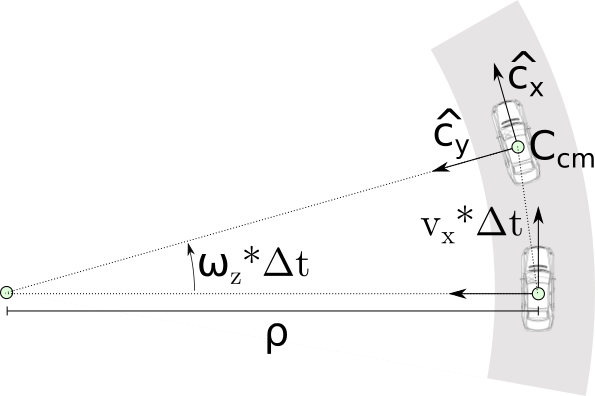
\includegraphics[width=0.95\linewidth]{car_drawing.png}
      \end{minipage}
    }
    %
    %
  \item Now assume the car travels at a constant forward speed
    ($\dot{v_x} = 0$) and does not slide ($v_y = \dot{v_y} = 0$). Using your
    result from (a), does constant speed imply zero acceleration?
    %
    \\[0.5pc]
    \Solution{}{1.0\linewidth}{
      \parbox{1.0\linewidth}{
        \begin{tabular}{l@{\equals[\;]}rcr}
            $\accel{\cm{C}}{N}$
          & $(0 \minus[\;] \omega_z * 0)~\uvecx{c}$
          & $\plus[\;]$
          & $(0 \plus[\;] \omega_z v_x)~\uvecy{c}$
          \\[0.5pc]
          & $0~\uvecx{c}$ & $\plus[\;]$ & $\omega_z v_x~\uvecy{c}$
        \end{tabular}
        \\[0.5pc]
        What does this result say? It says the \cm{C} has non-zero acceleration
        as long as there is simultaneously a non-zero speed and a non-zero rate of
        rotation, \textbf{even if they are both constant (not changing)}.
        \\[0.5pc]
        Note that if we do the substitution $w_z = v_x / \rho$ based on the
        scenario in (b), then we get
        \\[0.0pc]
        $$\accel{\cm{C}}{N} \equals[\;] (\frac{v_x}{\rho}) v_x~\uvecy{c}
          \equals[\;] \frac{v_x^2}{\rho}~\uvecy{c}$$
        Dotting with \uvecy{c} gives the magnitude of ``centripetal" acceleration,
        which will be familiar from introductory physics.
      }  % end parbox
    }  % end Solution
  %
  %
  %
\end{enumerate}

\isolatedBuildFooter
